%%%%%%%%%%%%%%%%%%%%%%%%%%%%%%%%%%%%%%%%%
% Short Sectioned Assignment
% LaTeX Template
% Version 1.0 (5/5/12)
%
% This template has been downloaded from:
% http://www.LaTeXTemplates.com
%
% Original author:
% Frits Wenneker (http://www.howtotex.com)
%
% License:
% CC BY-NC-SA 3.0 (http://creativecommons.org/licenses/by-nc-sa/3.0/)
%
%%%%%%%%%%%%%%%%%%%%%%%%%%%%%%%%%%%%%%%%%

%----------------------------------------------------------------------------------------
%	PACKAGES AND OTHER DOCUMENT CONFIGURATIONS
%----------------------------------------------------------------------------------------

\documentclass[paper=a4, fontsize=11pt]{scrartcl} % A4 paper and 11pt font size

\usepackage[T1]{fontenc} % Use 8-bit encoding that has 256 glyphs
\usepackage{fourier} % Use the Adobe Utopia font for the document - comment this line to return to the LaTeX default
\usepackage[english]{babel} % English language/hyphenation
\usepackage{amsmath,amsfonts,amsthm} % Math packages

\usepackage{lipsum} % Used for inserting dummy 'Lorem ipsum' text into the template

\usepackage{sectsty} % Allows customizing section commands
\allsectionsfont{\normalfont\scshape} % Make all sections centered, the default font and small caps
\usepackage{graphicx}
\usepackage{float}
\usepackage{fancyhdr} % Custom headers and footers
\pagestyle{fancyplain} % Makes all pages in the document conform to the custom headers and footers
\fancyhead{} % No page header - if you want one, create it in the same way as the footers below
\fancyfoot[L]{} % Empty left footer
\fancyfoot[C]{} % Empty center footer
\fancyfoot[R]{\thepage} % Page numbering for right footer
\renewcommand{\headrulewidth}{0pt} % Remove header underlines
\renewcommand{\footrulewidth}{0pt} % Remove footer underlines
\setlength{\headheight}{13.6pt} % Customize the height of the header

\numberwithin{equation}{section} % Number equations within sections (i.e. 1.1, 1.2, 2.1, 2.2 instead of 1, 2, 3, 4)
\numberwithin{figure}{section} % Number figures within sections (i.e. 1.1, 1.2, 2.1, 2.2 instead of 1, 2, 3, 4)
\numberwithin{table}{section} % Number tables within sections (i.e. 1.1, 1.2, 2.1, 2.2 instead of 1, 2, 3, 4)

\setlength\parindent{0pt} % Removes all indentation from paragraphs - comment this line for an assignment with lots of text

%----------------------------------------------------------------------------------------
%	TITLE SECTION
%----------------------------------------------------------------------------------------

\newcommand{\horrule}[1]{\rule{\linewidth}{#1}} % Create horizontal rule command with 1 argument of height

\title{	
\normalfont \normalsize 
\textsc{John A. Paulson School of Engineering and Applied Sciences} \\ [25pt] % Your university, school and/or department name(s)
\horrule{0.5pt} \\[0.4cm] % Thin top horizontal rule
\huge Project Update - CS287 \\ % The assignment title
\horrule{2pt} \\[0.5cm] % Thick bottom horizontal rule
}

\author{Nicolas Drizard \& Virgile Audi\\
nicolas.drizard@g.harvard.edu\quad vaudi@g.harvard.edu} % Your name

\date{\normalsize\today} % Today's date or a custom date

\begin{document}

\maketitle % Print the title

%----------------------------------------------------------------------------------------
% Introduciton %----------------------------------------------------------------------------------------

\section*{Introduction}

The focus of this final project is about non-factoid question answering. To solve the problem on non-factoid QA, we chose to implement memory network type of models and in particular the dynamic memory network presented in \cite{dmn}. For this first project update, we mainly worked on pre-processing the data form the bAbi dataset, implement a count-base baseline as well as looking at a one hop memory weakly supervised memory network.


%------------------------------------------------

\section{Pre-processing}

The goal of testing the created models on the bAbi dataset is to be able to have a model that works on all 20 pre-defined tasks without having to fine tune the prediction step. This constrain impacted the choice of pre-processing we adopted for this project. We wanted to create a pre-processing script that given a set of tasks and their respective training and test sets, would output a unique format of input and output data.\\

The first step of the pre-processing was to create a mapping between words present in the training and test sets and an index, and vice-versa. A particularity of the bAbi dataset is that even though it is not a Multiple Choice QA dataset, the number of possible answers is not infinite. We therefore decided to create mappings that given a set of tasks to solve, would start by indexing the words that appear as answers followed by the other words present in training and test stories and questions.\\

Given the tasks and the mappings mentioned above, the pre-processing script returns four matrices. The first matrix contains the sentences of the different stories using a bag of words representation, as well as the index of the task it belongs to. In this matrix, we concatenate the stories from all the inputed tasks, and sentences are therefore globally indexed and the index of a sentence in a story is disregarded. Using a similar trick as the one used in homework 1, we introduced padding in order to get a standard sentence size equal to the length of the longest sentence in training and testing.\\

We used the same construction for the second matrix that corresponds to the bag of words representation of the questions. We also output a vector that contains the index of the answers of the question. Finally we created a fourth matrix that maps the questions to the relevant sentences in the stories matrix. Each row of this matrix contains:

\begin{itemize}
\item the index of the first sentence of the corresponding story in the stories matrix,
\item the index of the last sentence of the corresponding story for this particular questions, 
\item the indices of the supporting facts in the stories matrix
\end{itemize}
The number of supporting facts might vary from task to task, and has a maximum of 3. If we are dealing with less than 3 facts, we fill the row with 0 entries.

\section{Count-Base Baseline}
\subsection{Model Presentation}

\paragraph{Question/Word embedding}
\paragraph{???}
\paragraph{Sentence Matching}

The count-model worked rather well just using the previous features. We felt never the less that implementing a first sentence matching step could help improve results. The goal of this step was to restrict the number of sentences in which we could find the answer to a given question. To do so, we used co-occurences of words in the questions with words in the sentences of the story. This is similar to the algorithm presented in the MCtest paper \cite{mct}. This step allows to look for one or more supporting facts. If the desired number of facts is one, the function outputs the highest scoring sentence on account of word co-occurences. Consider the following example:\\
\begin{center}
Mary picked up the football.\\
Mary went to the garden.\\
John walked to the garden.\\
Where is the football?
\end{center}
If we look for more than one supporting fact, then word counts would not help us answer the question, as the only scoring sentence (if we disregard stop words such as the) would be the first sentence. So the function we coded uses an iterative approach to narrow the search for supporting facts. It then looks for sentences that have co-occurences with the sentences that scored in the first question/sentence matching. The fact that "Mary" appears both in the first and second sentence will allow us to return the relevant facts to answering the question.\\

A potential downside to this method is that it will most of the time find more than three supporting facts which is the maximum amount of supporting facts needed to answer questions of any tasks. Nevertheless, this step would only be necessary for the count-base model. And since the use of this model was just to act as a baseline to the memory networks, we decided that the model performed sufficiently well to leave it to that.

\subsection{Results}
\section{Memory Network}

If we didn't have sufficient time to implement a first memory network, we wanted to present the first memory network we will implement. The model was introduced in \cite{mem} and can be summarised in the following graphical representation:

\begin{figure}[H]
\begin{center}
    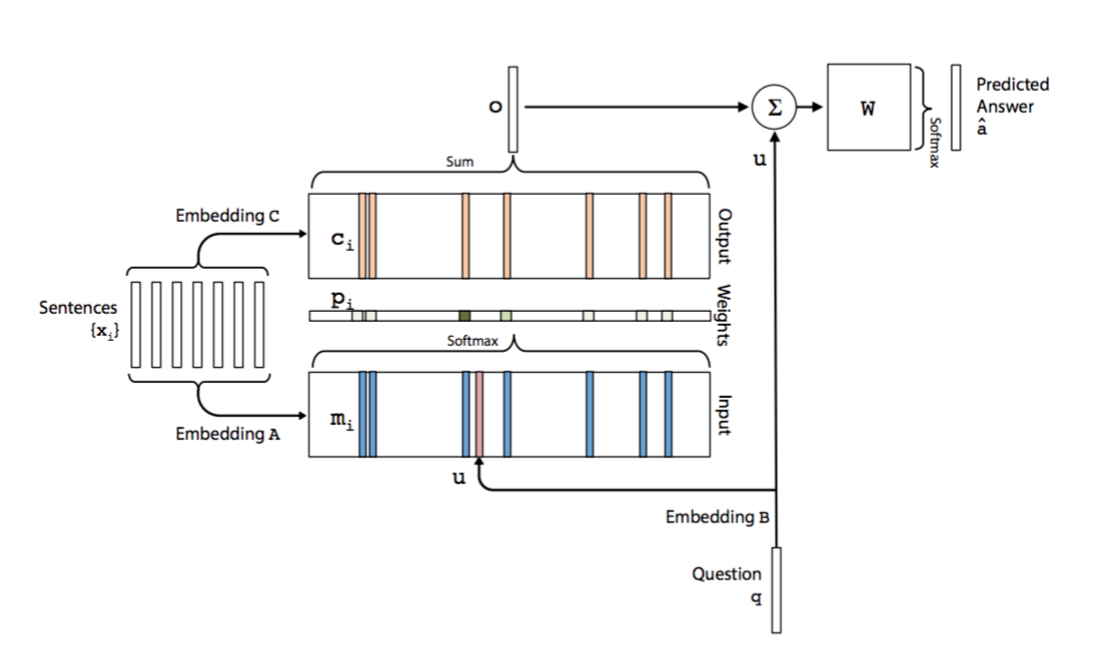
\includegraphics[width=0.7\textwidth]{mem.png}
    \caption{1-Hop Memory Network}
\end{center}
\end{figure}

This model implements a single memory hop operation. This model takes for inputs the question and the sentences of the story. The sentences of the story are then embedded with two differents look-up tables. The first look-up table (which corresponds to the matrix A in the above diagram) will be used to store the sentences of the stories as input in memory. These embedded representation of the story's sentences will then be combined with the embedded representation of the question (using the matrix B) using a dot product. The result of this dot product is then passed through a softmax layer to give a probability distribution over which sentence is likely to give information about the answer. The memory output vector $o$ results from a weighted sum of the output embeddings of the sentences (using matrix C) using the probability distribution $p$. We then apply a weight matrix to the sum of question embeddings and the output vector $o$ followed by a softmax to predict the answer. We can summarize this process with the formula:

$$\hat{a} = \text{softmax}\left(W(o+u)\right)$$
where: $ o = \sum\limits_{i=1}\text{softmax}(u^Tm_i)$, with $u$ being the embedded representation of the question and $m_i$ the embedded represenation of the sentence $i$ in the story.\\

The embedded representation of sentences and questions can either be obtained by summing the embeddings of their words or by concatenating them. We plan on testing the two approaches.\\

Finally, we will implement a temporallity feature by modifying the embedded representation of the sentences by adding a term depending on the index of the sentence in the story.

\section{Future Steps}

If we plan to code this model using the regular "nn" module, we would also like to use the "nngraph" module. Indeed, once this model implemented, we would like to implement a variation by adding mutliple hops to memory. This model is also presented in \cite{mem} and its structure could be too complex for the "nn" module. We will then tackle the dynamic memory network that we introduced in the proposal and can be found in \cite{dmn}.
%----------------------------------------------------------------------------------------
\bibliographystyle{apalike}
\bibliography{update}
\end{document}